\subsection{Problem}

\renewcommand{\theequation}{\theenumi}
\begin{enumerate}[label=\thesection.\arabic*.,ref=\thesection.\theenumi]
\numberwithin{equation}{enumi}
	\item Two rails are represented as 
	\begin{multline}
	\myvec{1&2}\vec{x}=4\text{ and }\myvec{2&4}\vec{x}=12.
	\end{multline}
	\quad Will the rails cross each other?
	
	\solution The above equations can be represented as a matrix equation as
	\begin{align}\myvec{1&2\\2&4}\vec{x}=\myvec{4\\12}\vec{x}\end{align}
	The augmented matrix for the above matrix is row reduced as follows:
	\begin{align}\myvec{1&2&4\\2&4&12}\xleftrightarrow {R_2\leftarrow \frac{R_2}{2}}\myvec{1 & 2 & 4\\1 & 2 & 6} \\
\xleftrightarrow {R_2\leftarrow R_2 - R_1}\myvec{1 & 2 & 4\\0 & 0 & 2}
\end{align}
	Thus the row reduction of the 2$\times$3 matrix 
	\begin{align}
		\myvec{1&2&4\\2&4&12}
	\end{align}
	results in a matrix with two non zero rows having rank 2. Similarly the rank is 1 for the matrix$\myvec{1&2\\2&4}$\\
	As the rank of these two matrices aren't same, there is no solution. Therefore, the rails don't cross over eachother.
	The following python code computes the area of $\triangle$ABC in Fig.\ref{fig:qfive}.
	\begin{lstlisting}
	./codes/lines/q5.py
	\end{lstlisting}
	\begin{figure}[!ht]
	\centering
	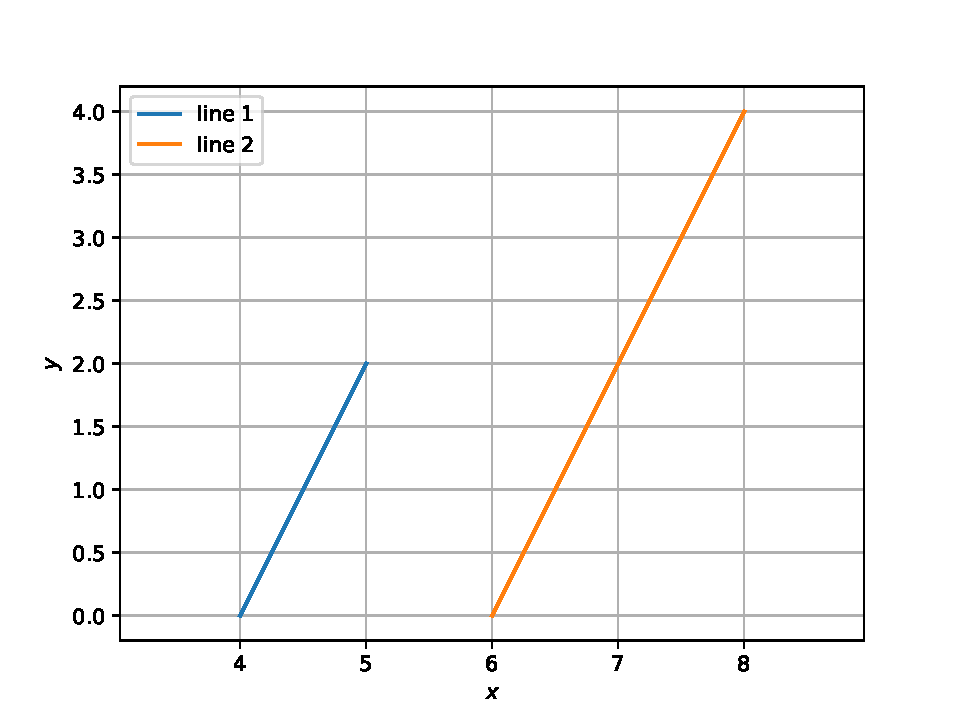
\includegraphics[width=\columnwidth]{./figs/lines/q5.pdf}
	\caption{Rails of Q.3.1.5}
	\label{fig:qfive}	
	\end{figure}
	
\end{enumerate}
